% --- ETUDE DE CAS ---
\section*{Étude de cas: Virtualisation}
\addcontentsline{toc}{section}{Étude de cas: Virtualisation}

\section*{AAV}
\addcontentsline{toc}{section}{AAV}
\begin{itemize}
  \item [2] Décrire le fonctionnement de la virtualisation
  \item [2] Décrire le fonctionnement de la conteneurisation
  \item [3] Expérimenter la conteneurisation
  \item [3] Administrer une architecture de virtualisation de serveurs
  \item [3] Automatiser la création d'un environnement virtuel
  \item [4] Comparer les différents types de virtualisation
  \item [5] Structurer un argumentaire sur le choix de virtualisation en fonction du contexte
  \item [3] Etablir un inventaire fonctionnel
  \item [2] Résumer l'intérêt d'un CMDB en entreprise au regard de la supervision
  \item [5] Réorganiser la sécurité d'une infrastructure
\end{itemize}

\subsection*{Mots clés}
\phantomsection
\addcontentsline{toc}{subsection}{Mots clés}
\begin{itemize}
  \item GLPI (Gestionnaire Libre de Parc Informatique)
  \item POC (Proof of Concept)
  \item ITSM (Information Technology Service Management)
  \item ITIL (Information Technology Infrastructure Library)
  \item VM (Virtual Machine)
  \item RDP (Remote Desktop Protocol)
  \item ESXi
  \item Cloud (Cloud Computing)
  \item Cluster Hyper-V
  \item CMDB (Configuration Management Database)
  \item Hyperviseur Bare-metal (Type 1)
  \item Docker
  \item Hyperviseur Type 2 (Hosted)
  \item SSH (Secure Shell)
  \item NAS (Network Attached Storage)
  \item Data Center (Centre de données)
\end{itemize}

\subsection*{Contexte}
\phantomsection
\addcontentsline{toc}{subsection}{Contexte}
Léa souhaite mettre en place son POC sur GLPI pour remplacer l’organisation actuelle avec Leila. Ils doivent choisir comment déployer l’outil : soit avec une VMC Classique, soit via des conteneurs docker.

\subsection*{Problématique}
\phantomsection
\addcontentsline{toc}{subsection}{Problématique}
Quelle est la meilleure façon de déployer GLPI sur la VM de test (VM, Docker).

\newpage

\subsection*{Contraintes}
\phantomsection
\addcontentsline{toc}{subsection}{Contraintes}
\begin{itemize}
  \item Serveur web-php
  \item Architecture GLPI
  \item Hyperviseurs (bare-metal)

\end{itemize}

\subsection*{Généralisation}
\phantomsection
\addcontentsline{toc}{subsection}{Généralisation}
\begin{itemize}
  \item Types de virtualisation

\end{itemize}

\subsection*{Livrables}
\phantomsection
\addcontentsline{toc}{subsection}{Livrables}
\begin{itemize}
  \item VM de tests
  \item Rapport détaillé ( Avantages / inconvénients | Plan de déploiement)
\end{itemize}

\subsection*{Pistes de solutions}
\phantomsection
\addcontentsline{toc}{subsection}{Pistes de solutions}
\begin{itemize}
  \item Étudier l'architecture de GLPI : Identifier les composants nécessaires (Web, BDD) pour dimensionner la demande.
  \item Se renseigner sur les différences entre VM et docker : Faire un tableau comparatif (avantages/inconvénients) entre une VM "monolithique" et l'usage de Docker, notamment sur les aspects performance et consommation (Green IT).
  \item Analyser l'hyperviseur Hyper-V : Comprendre le fonctionnement d'un hyperviseur de type 1 et comment s'y intègre une VM Linux.
  \item e renseigner sur le déploiement Docker : Rechercher comment déployer une stack LAMP (Linux Apache MySQL PHP) via Docker et docker-compose.
\end{itemize}

\subsection*{Plan d'action}
\phantomsection
\addcontentsline{toc}{subsection}{Plan d'action}
\begin{itemize}
  \item Définir les mots clés
  \item Etudier les ressources
  \item Etudier le fonctionnement de GLPI
  \item Analyser le fonctionnement technique de la virtualisation
  \item Comprendre les principes et le fonctionnement de la conteneurisation
  \item Comparer les deux approches (VM vs Conteneurs) dans le contexte du projet (ressources, maintenance, Green IT)
  \item Lister les prérequis techniques pour l'installation de GLPI.
  \item Choisir et déployer l'architecture cible (OS de la VM + méthode d'installation de l'appli)
  \item Rédiger les spécifications pour la demande de VM (CPU, RAM, Stockage, OS)
\end{itemize}

\section*{Démarche~: Virtualisation}
\addcontentsline{toc}{section}{Démarche~: Virtualisation}

\subsection*{Définition: Mots clés}
\phantomsection
\addcontentsline{toc}{subsection}{Définition: Mots clés}

\textbf{GLPI (Gestionnaire Libre de Parc Informatique)}
GLPI est une solution open-source destinée à la gestion complète d'un parc informatique.
\begin{center}
  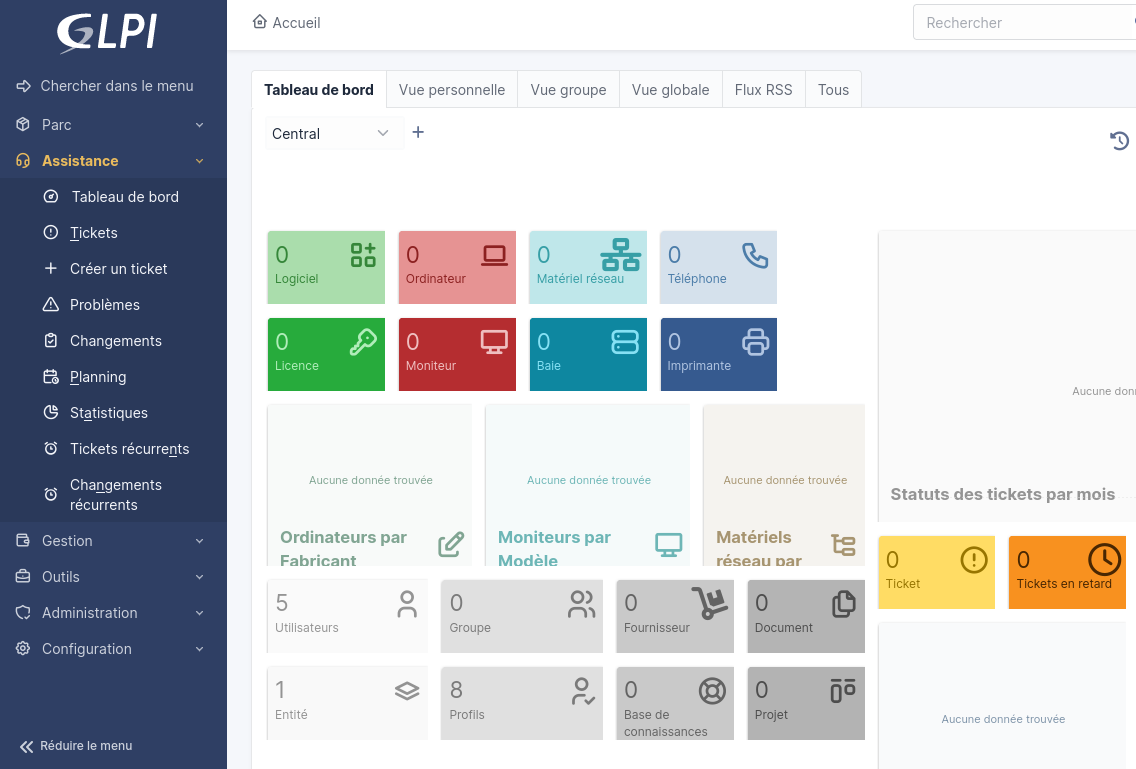
\includegraphics[width=0.8\linewidth]{contents/img/Glpi.png}
\end{center}
Elle centralise l'inventaire matériel et logiciel grâce à des agents installés sur les postes et serveurs, permet la gestion des incidents et des demandes via un système de tickets, et administre le cycle de vie des équipements. GLPI inclut également un module de CMDB offrant une vision globale des éléments d'infrastructure et de leurs relations. Cet outil est largement utilisé pour structurer les services ITSM et améliorer la traçabilité opérationnelle.

\textbf{POC (Proof of Concept)}
Un POC est une expérimentation ciblée visant à démontrer la faisabilité technique ou fonctionnelle d'une solution. L'objectif n'est pas de produire un livrable final, mais de valider les capacités de la technologie en termes de performance, de compatibilité, de sécurité ou d'intégration. Le POC réduit fortement les risques projets et sert souvent de base décisionnelle pour le passage en phase de déploiement.

\textbf{ITSM (Information Technology Service Management)}
L'ITSM regroupe l'ensemble des processus, méthodes et outils permettant de gérer les services informatiques tout au long de leur cycle de vie. 

\begin{center}
  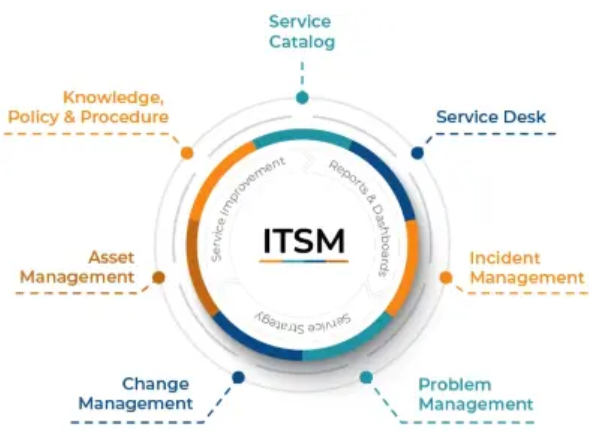
\includegraphics[width=0.7\linewidth]{contents/img/ITSM.png}
\end{center}

Cette approche structurée organise la gestion des incidents, des demandes, des problèmes et des changements, tout en encadrant la qualité de service via des objectifs mesurables comme les SLA. L'ITSM vise à aligner les services informatiques sur les enjeux métier.

\textbf{ITIL (Information Technology Infrastructure Library)}
ITIL est un corpus international de bonnes pratiques destiné à structurer l'organisation et le fonctionnement d'une DSI. Il propose un modèle complet pour gérer efficacement les services IT, incluant la gestion des incidents, des changements, des problèmes, des configurations, ainsi que les processus de disponibilité et de continuité opérationnelle. ITIL sert de référence pour améliorer la maturité d'une organisation informatique.

\textbf{Machine virtuelle (VM)}
Une machine virtuelle est un environnement informatique isolé exécuté au-dessus d'un hyperviseur. Elle embarque son propre système d'exploitation, ses ressources dédiées (CPU, RAM, stockage) et fonctionne indépendamment des autres VM. Grâce à la mutualisation du matériel, à la flexibilité de déploiement et aux fonctions avancées (snapshots, migrations), les VM constituent la base des infrastructures modernes.

\textbf{RDP (Remote Desktop Protocol)}
RDP est un protocole Microsoft permettant la prise de contrôle graphique d'un poste Windows à distance. Il transmet l'affichage, les actions clavier/souris et peut rediriger des périphériques comme les disques ou imprimantes. Dans les environnements professionnels, il est indispensable pour l'administration à distance et le support des utilisateurs.

\textbf{ESXi}
ESXi est l'hyperviseur bare-metal de VMware. Installé directement sur un serveur physique, il permet d'héberger et de gérer des machines virtuelles avec des fonctionnalités avancées telles que vMotion, High Availability, DRS ou les snapshots. Il constitue l'une des solutions de virtualisation les plus répandues dans les datacenters.

\newpage

\textbf{Cloud Computing}
Le Cloud Computing désigne la fourniture de ressources informatiques à la demande via Internet. Il inclut le provisionnement de machines virtuelles, de conteneurs, de services managés, de stockage ou d'outils DevOps. Ces ressources sont élastiques, facturées à l'usage et accessibles via API. Les principaux fournisseurs sont AWS, Azure et Google Cloud Platform.

\textbf{Cluster Hyper-V}
Un cluster Hyper-V est un ensemble de serveurs Windows configurés pour assurer une haute disponibilité des machines virtuelles. Grâce à un stockage partagé et à la gestion du cluster de basculement, les VM peuvent migrer automatiquement vers un autre nœud en cas de panne. Ce mécanisme garantit la continuité des services hébergés.

\textbf{CMDB (Configuration Management Database)}
La CMDB est la base de données centralisant la description de tous les composants du système d'information : serveurs, applications, services, flux et relations entre éléments. Elle permet d'identifier les dépendances, d'évaluer l'impact d'un changement et de faciliter le diagnostic lors d'incidents. Une CMDB fiable est essentielle pour les organisations alignées sur ITIL.

\textbf{Hyperviseur Bare-Metal (Type 1)}
Un hyperviseur de type 1 s'installe directement sur le matériel physique sans système d'exploitation intermédiaire. Cette architecture offre de meilleures performances, une sécurité renforcée et une stabilité accrue. Les principales solutions de ce type incluent VMware ESXi, Hyper-V Server et Proxmox.

\textbf{Docker}
Docker est une technologie de conteneurisation permettant d'exécuter une application dans un environnement isolé, léger et reproductible. Les conteneurs empaquent l'application et ses dépendances, garantissant une compatibilité parfaite entre environnements. Docker est devenu un outil incontournable pour le déploiement agile, les architectures microservices et les pipelines DevOps.

\textbf{Hyperviseur Type 2 (Hosted)}
Un hyperviseur de type 2 fonctionne au-dessus d'un système d'exploitation hôte. Bien que moins performant qu'un hyperviseur bare-metal, il est simple à mettre en place et largement utilisé pour les environnements de test ou de développement. Des exemples courants sont VirtualBox et VMware Workstation.

\textbf{SSH (Secure Shell)}
SSH est un protocole sécurisé permettant l'accès distant à un système via une interface en ligne de commande. Il chiffre l'ensemble des communications, offre un mécanisme d'authentification par clés et permet l'exécution de commandes distantes, ainsi que le transfert de fichiers via SCP ou SFTP. C'est l'outil central pour l'administration des systèmes Linux.

\textbf{NAS (Network Attached Storage)}
Un NAS est un équipement de stockage réseau autonome. Il fournit des partages accessibles en SMB ou en NFS, gère la redondance via des configurations RAID, et permet la sauvegarde ou la réplication des données. Il est couramment utilisé pour le stockage centralisé dans les PME ou les projets internes.

\textbf{Datacenter}
Un datacenter est un site physique conçu pour héberger des infrastructures informatiques dans un environnement sécurisé et contrôlé. Il fournit une alimentation redondée, une climatisation adaptée, une connectivité réseau de haute capacité et des dispositifs de sécurité physique. Les serveurs, baies de stockage, clusters et équipements critiques y sont regroupés pour garantir un fonctionnement continu.

\newpage

\section*{Cours et ressources utilisées}
\addcontentsline{toc}{section}{Cours et ressources utilisées}

\subsection*{Installation de Docker}
\phantomsection
\addcontentsline{toc}{subsection}{Installation de Docker}
\noindent Installez les paquets nécessaires à l'installation de Docker
\begin{verbatim}
  sudo apt-get install  curl apt-transport-https ca-certificates
  software-properties-common
\end{verbatim}

Questions~:
Quels sont les paquets installés et pourquoi ?
\begin{itemize}
  \item curl : outil de transfert de données
  \item apt-transport-https : permet à APT d'utiliser des dépôts via le protocole HTTPS
  \item ca-certificates : gère les certificats SSL pour sécuriserles connexions
  \item software-properties-common : fournit des outils pour gérer les sources de logiciels
\end{itemize}

\subsection*{Ajouter la clé GPG}
\phantomsection
\addcontentsline{toc}{subsection}{Ajouter la clé GPG}
\noindent Vous allez ajouter le dépôt docker mais tout d'abord exécutez les deux lignes de commande suivante.

\begin{verbatim}
  sudo mkdir -m 0755 -p /etc/apt/keyrings
  curl -fsSL https://download.docker.com/linux/ubuntu/gpg |
  sudo gpg --dearmor -o /etc/apt/keyrings/docker.gpg
\end{verbatim}

\noindent GPG est un logiciel open source gratuit basé sur le standard de cryptographie à clé publique PGP. \\
Les dépôts logiciels utilisent des clés GPG pour signer les paquets. Lorsqu'APT télécharge un paquet, il vérifie la signature du paquet en utilisant la clé GPG correspondante. Cela garantit que les paquets proviennent d'une source fiable et qu'ils n'ont pas été modifiés. Ajouter la clé GPG assure que les paquets Docker que vous allez télécharger et installer sont authentiques et n'ont pas été altérés.
\begin{itemize}
  \item La première commande créé un répertoire utilisé pour stocker les clés GPG des dépôts APT.
  \item La deuxième commande télécharge et convertir la clé GPG au format binaire.
\end{itemize}

\newpage

\subsection*{Ajout du dépôt officiel de Docker}
\phantomsection
\addcontentsline{toc}{subsection}{Ajout du dépôt officiel de Docker}
\noindent Vous allez maintenant ajouter le dépôt officiel de Docker à la liste des sources APT de votre système Ubuntu. Voici la commande :

\begin{verbatim}
  echo "deb [arch=$(dpkg --print-architecture) signed-by=/etc/apt/keyrings
  /docker.gpg] https://download.docker.com/linux/ubuntu $(lsb_release -cs)
  stable" | sudo tee /etc/apt/sources.list.d/docker.list > /dev/null
\end{verbatim}

Questions~:\\
Cherchez à comprendre ce que font ces commandes. Pourquoi /dev/null ?\\
Qu'est-ce que /etc/apt/sources.list.d/docker.list ?\\
Qu'indique signed-by=/etc/apt/keyrings/docker.gpg ?\\

\begin{itemize}
  \item La commande echo crée une nouvelle entrée de dépôt pour Docker.
  \item dpkg --print-architecture : récupère l'architecture du système (amd64, arm64, etc.)
  \item lsb\_release -cs : récupère le nom de code de la version d'Ubuntu installée.
  \item signed-by=/etc/apt/keyrings/docker.gpg : indique à APT d'utiliser cette clé GPG pour vérifier les paquets provenant de ce dépôt.
  \item sudo tee /etc/apt/sources.list.d/docker.list : écrit la sortie de la commande echo dans un nouveau fichier de liste de sources APT spécifique à Docker.
  \item > /dev/null : redirige la sortie standard vers /dev/null pour éviter d'afficher le contenu dans le terminal.
\end{itemize}

\subsection*{Installation de Docker}
\phantomsection
\addcontentsline{toc}{subsection}{Installation de Docker}
\noindent Maintenant vous allez installer Docker

\begin{verbatim}
  sudo apt-get update
  sudo apt-get install docker-ce docker-ce-cli containerd.io
  docker-buildx-plugin docker-compose-plugin
\end{verbatim}

Cette commande installe :
\begin{itemize}
  \item Docker Community Edition : Le moteur Docker principal pour exécuter des conteneurs.
  \item Docker CLI : Les outils en ligne de commande pour interagir avec Docker.
  \item Containerd : Le moteur de conteneurisation utilisé par Docker pour gérer les conteneurs.
  \item Buildx Plugin : Pour construire des images de conteneurs avec des fonctionnalités avancées.
  \item Compose Plugin : Pour orchestrer des applications multi-conteneurs.
\end{itemize}

Vérifiez si tout va bien avec la commande \texttt{sudo systemctl status docker}

\begin{center}
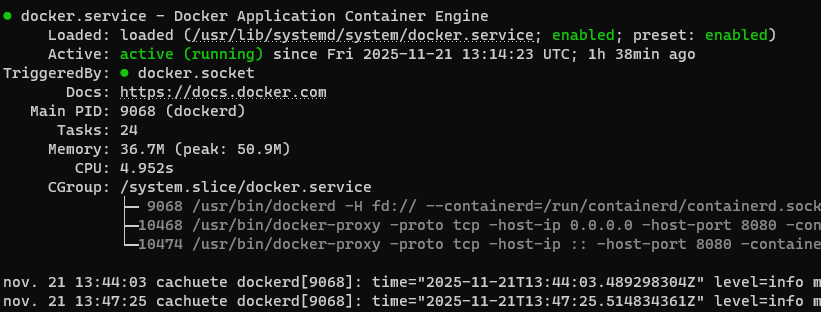
\includegraphics[width=0.8\textwidth]{contents/img/docker_statut.png}
\end{center}

\section*{Corbeille d'Excercice}
\addcontentsline{toc}{section}{Corbeille d'Excercice}

\noindent Hyper-V est un rôle qui peut être installé sur un serveur Windows mais aussi sur un PC Windows 10 ou
11.

\noindent Cette corbeille utilise la virtualisation imbriquée (ou nested virtualization) : Installer un hyperviseur (Hyper-V) dans une machine virtuelle VMware.

\noindent La version de VMware doit être supérieure à la version 15 (c'est le cas).

\noindent La virtualisation imbriquée, très pratique quand on veut réaliser des tests mais elle ne doit jamais être utilisée en production.

\noindent Les serveurs Hyper-V en production sont souvent installés en mode Core. Il est donc important de savoir les administrer sans interface graphique (même si, souvent, ils sont administrés graphiquement à distance via des Outils d’administration ou via Windows Admin Center)

\noindent Windows Server Core améliore la sécurité du système en réduisant le nombre de composants installés

\subsection*{PRESENTATION DE MICROSOFT HYPER-V}
\phantomsection
\addcontentsline{toc}{subsection}{PRESENTATION DE MICROSOFT HYPER-V}
\noindent \textbf{Hyper-V est un hyperviseur développé par Microsoft} et introduit à Windows pour la première fois en 2008. La solution de virtualisation Hyper-V est intégrée dans Windows Server, depuis Windows Server 2008 et est également disponible dans certaines éditions de Windows 10 et Windows 11. Pour être plus précis, Windows 8 a été la première version à permettre l'installation d'Hyper-V sur un poste de travail.

\noindent Que ce soit dans Windows ou Windows Server, il est important de noter qu'\textbf{Hyper-V est intégré, mais qu'il n'est pas installé par défaut.}

\newpage

\noindent Hyper-V présente l'avantage d'être intégré dans Windows, ce qui signifie qu'il peut être plus facile à gérer pour les organisations qui utilisent déjà Windows Server. Ces mêmes organisations qui ont déjà potentiellement une maitrise technique de ce système d'exploitation.

\noindent Hyper-V est un hyperviseur stable qui a fait ses preuves depuis de nombreuses années.
\begin{itemize}
  \item Avec une licence Windows Server 2022 Standard, vous avez le droit de créer 2 machines virtuelles,
  \item Avec une licence Windows Server 2022 Datacenter, vous avez le droit de créer un nombre illimité de VM.
\end{itemize}

\noindent \textbf{Hyperviseur de type 1, Hyper-V s'exécute directement sur le matériel et offre des performances
élevées, comparables à celles de concurrents comme VMware ESXi.}

\noindent VMware ESXi est souvent considéré comme légèrement plus riche en fonctionnalités pour les déploiements d'entreprise à grande échelle et n'utilise pas un environnement centré sur Microsoft.

\subsection*{Prérequis}
\phantomsection
\addcontentsline{toc}{subsection}{Prérequis}
\noindent Vous avez besoin de :
\begin{itemize}
  \item Une VM serveur Windows 2022, installation de base comme décrite dans la séquence de préparation.
  \item Le fichier ISO d'installation de Ubuntu.
\end{itemize}

\noindent Votre PC physique à accès à Internet.

\noindent Pensez à arrêter vos autres VM pour économiser mémoire et processeur.

\noindent Attention : Cet environnement dit ‘nested’ est totalement déconseillé en \textbf{production}, mais reste fonctionnel pour un environnement de test.

\noindent Cependant, pour des raisons matérielles imprévisibles (chaque élève a son propre matériel), un environnement 'nested' peut ne pas fonctionner, ce qui ne vous empêche pas de lire le contenu ou de travailler en binôme.

\newpage

\subsection*{Architecture nécessaire}
\phantomsection
\addcontentsline{toc}{subsection}{Architecture nécessaire}
\noindent Voici le schéma de l'utilisation de la virtualisation imbriquée (Nested)

\noindent
\begin{figure}[h!]
\centering
\begin{minipage}[t]{0.36\textwidth}
  \vspace{0pt} % aligne parfaitement en haut
  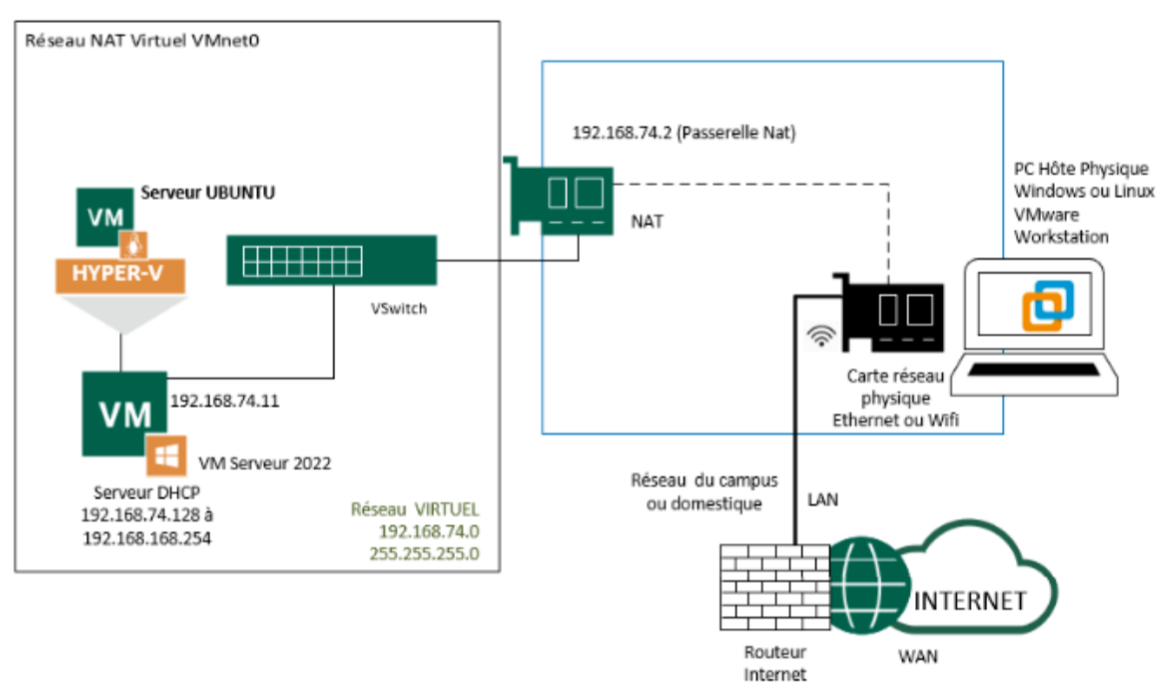
\includegraphics[width=\linewidth]{contents/img/architecture.png}
\end{minipage}
\hfill
\begin{minipage}[t]{0.62\textwidth}
  \vspace{0pt} % aligne parfaitement en haut
  Vous avez un hyperviseur de type 2 sur votre PC physique : VMware Workstation Pro.\\[6pt]
  Cet hyperviseur héberge une machine virtuelle Windows Server 2022, dans laquelle est installé un hyperviseur de type 1, Microsoft Hyper-V.\\[6pt]
  Cette machine virtuelle Windows Server 2022 va elle-même héberger une machine virtuelle Ubuntu Server.
\end{minipage}
\end{figure}


\noindent Hyper-V prend en charge plusieurs versions des distributions Windows Server, Windows et Linux, pour s'exécuter sur des machines virtuelles, en tant que systèmes d'exploitation invités.

\subsection*{Paramétrage}
\phantomsection
\addcontentsline{toc}{subsection}{Paramétrage}
1. Vous avez une VM Windows 2022 avec
\begin{itemize}
  \item une interface réseau sur VMnet0 NAT
  \item 4 Go de mémoire vive
\end{itemize}

2. Activez la virtualisation imbriquée dans la configuration de cette VM. \\
La virtualisation imbriquée dans VMware Workstation est désactivée par défaut. Elle s'active VM par VM. \\
L'objectif va être d'exposer les fonctions de virtualisation, notamment l'Intel VT-x ou l'AMD-V selon votre type de processeur, directement au sein de la machine virtuelle

\noindent 1. Arrêter la VM \\
2. Ouvrez les \textbf{Virtual Machine Settings} choisissez dans l'onglet \textbf{Hardware > Processors}. Cochez \textbf{"Virtualize Intel VT-x/EPT or AMD-V/RVI"}.

% --- Mémoire VM ---
\noindent
\begin{minipage}[t]{0.36\textwidth}
  \vspace{0pt}
  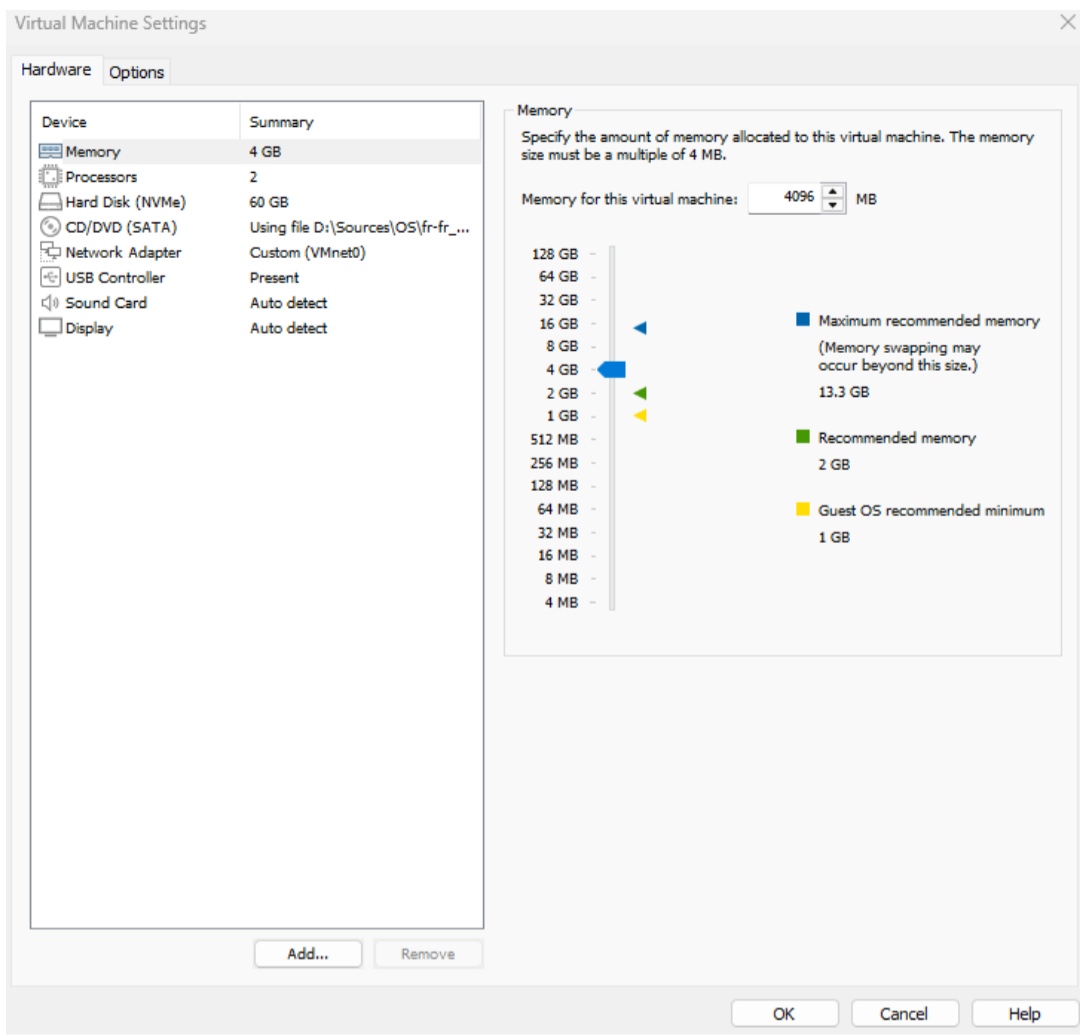
\includegraphics[width=\linewidth]{contents/img/VM_memory.png}
\end{minipage}
\hfill
\begin{minipage}[t]{0.62\textwidth}
  \vspace{0pt}
  Ouvrez les \textbf{Virtual Machine Settings} puis l'onglet \textbf{Hardware > Memory}.\\[6pt]
  Configurez \textbf{Memory for this virtual machine} à \textbf{4096 MB}.
\end{minipage}

\vspace{10pt}

% --- Processeurs VM ---
\noindent
\begin{minipage}[t]{0.36\textwidth}
  \vspace{0pt}
  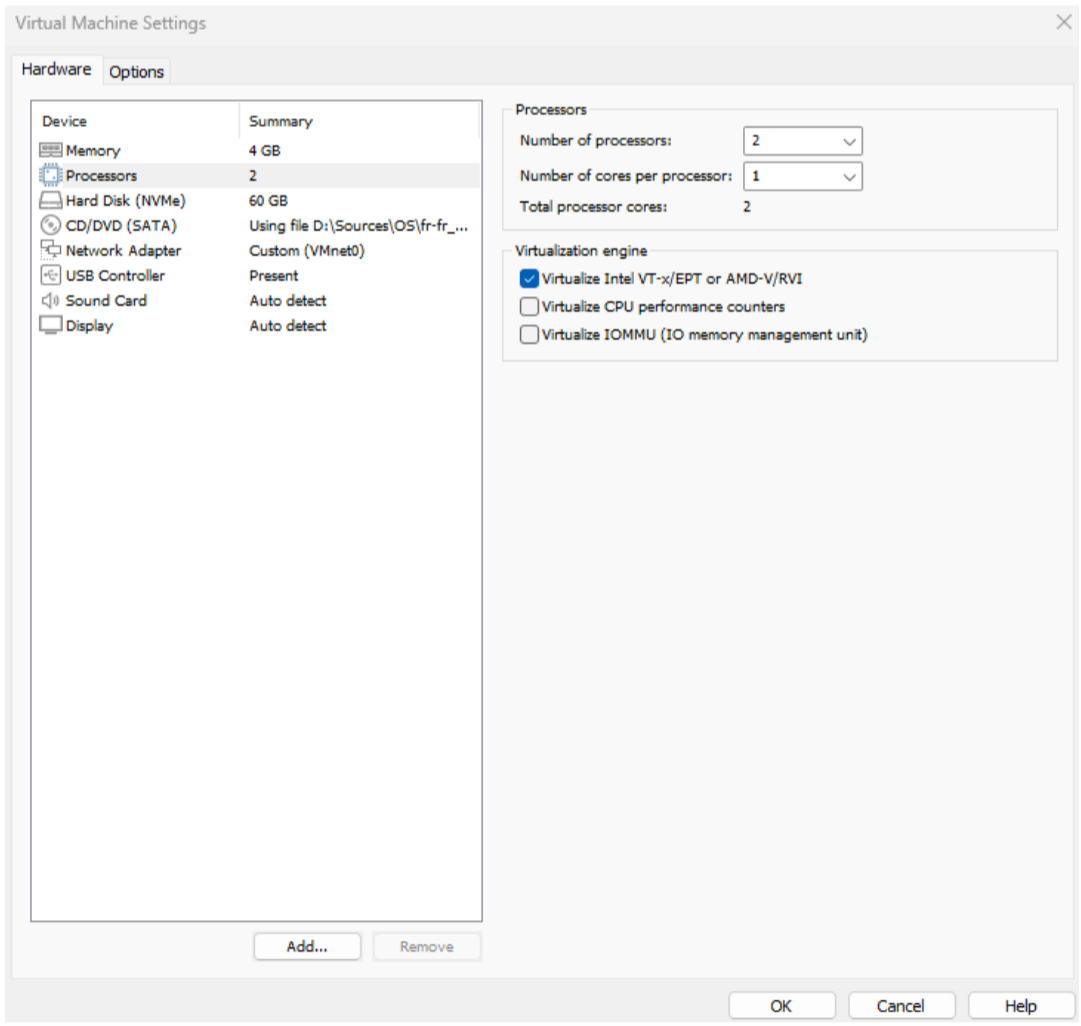
\includegraphics[width=\linewidth]{contents/img/VM_processors.png}
\end{minipage}
\hfill
\begin{minipage}[t]{0.62\textwidth}
  \vspace{0pt}
  Ouvrez les \textbf{Virtual Machine Settings} puis l'onglet \textbf{Hardware > Processors}.\\[6pt]
  Cochez l'option \textbf{"Virtualize Intel VT-x/EPT or AMD-V/RVI"}.
\end{minipage}

\vspace{10pt}

% --- Carte réseau VM ---
\noindent
\begin{minipage}[t]{0.36\textwidth}
  \vspace{0pt}
  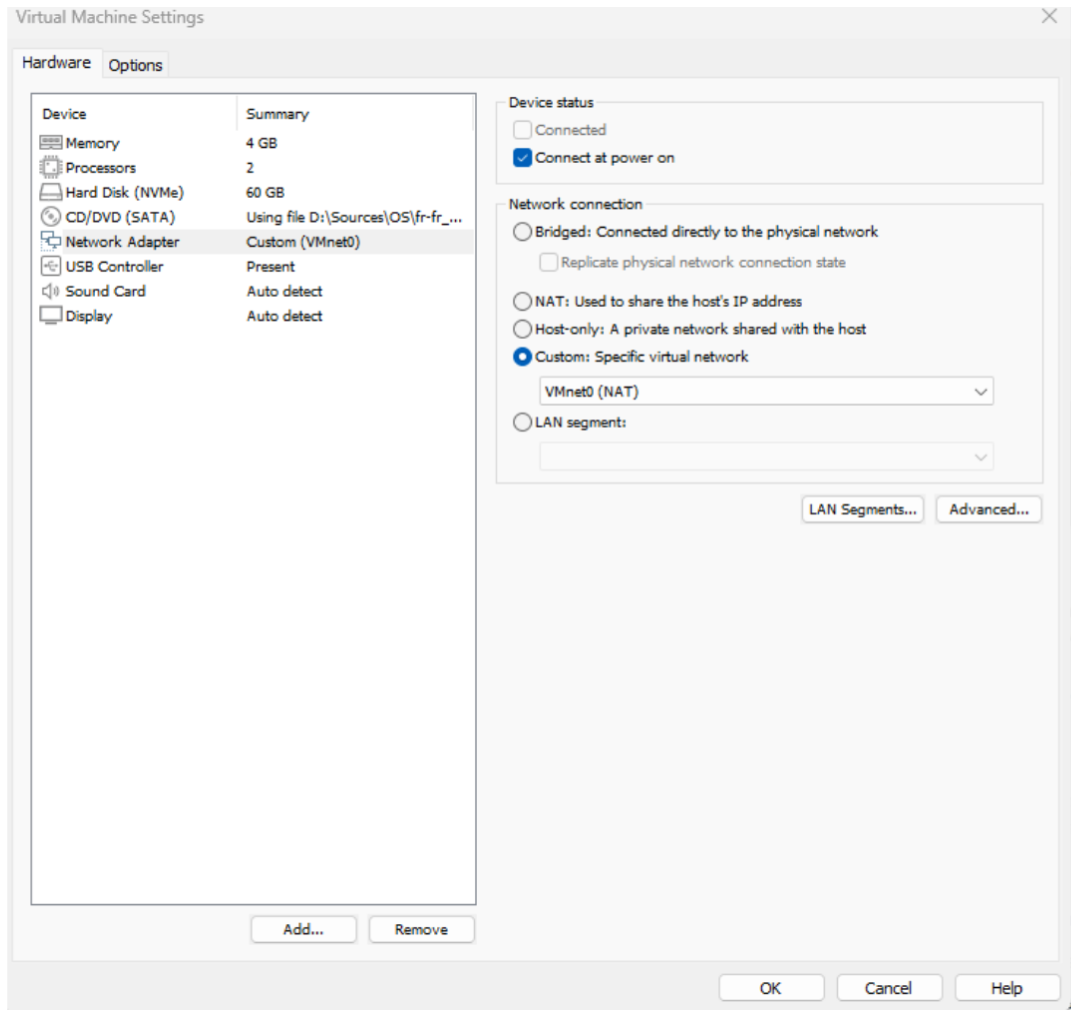
\includegraphics[width=\linewidth]{contents/img/VM_network.png}
\end{minipage}
\hfill
\begin{minipage}[t]{0.62\textwidth}
  \vspace{0pt}
  Ouvrez les \textbf{Virtual Machine Settings} puis l'onglet \textbf{Hardware > Network Adapter}.\\[6pt]
  Sélectionnez \textbf{Custom} et choisissez \textbf{VMNet0 (NAT)}.
\end{minipage}

\vspace{10pt}

% --- Configuration IP ---
\noindent En exécutant la commande \textbf{IPCONFIG} dans la VM Windows Server 2022, vous devez obtenir :\\[6pt]
\begin{itemize}
  \item Une adresse IP fixe pour l'interface réseau.
  \item Une adresse de passerelle.
\end{itemize}
\begin{center}
  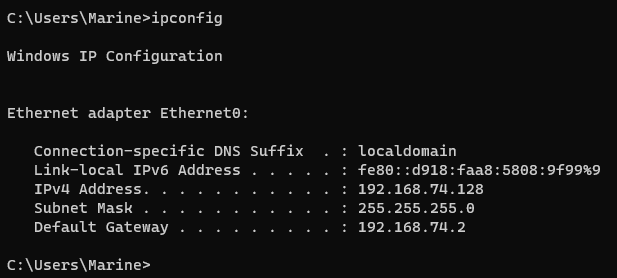
\includegraphics[width=0.7\linewidth]{contents/img/ipconfig.png}
\end{center}

Testez la connectivité conformément à la séquence de préparation.\\[6pt]
Exemple :
\begin{verbatim}
  ping <adresse_passerelle>
  ping google.com
\end{verbatim}

\newpage

Questions~: \\
Vous n'arrivez pas à démarrer la VM Windows 2022, vous ne pouvez pas faire de virtualisation imbriquée. \\
Vous avez une erreur : 

\begin{center}
  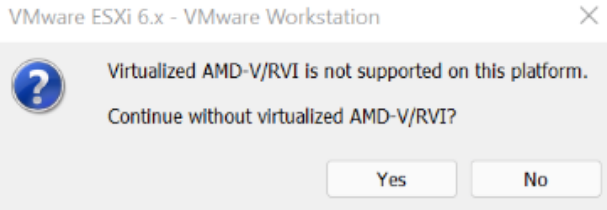
\includegraphics[width=0.5\linewidth]{contents/img/error_esxi6.png}
\end{center}

\noindent Solution 1: \textbf{ Modifier le paramétrage de l'hôte (votre PC)}\\
Appliquez les préconisation de cet Article de la base de connaissance Broadcom : \url{https://knowledge.broadcom.com/external/article?legacyId=2146361}

\noindent Solution 2: \textbf{ Si votre PC est sous Windows 10-11, installez Hyper-V sur votre PC}\\
Hyper-V peut cohabiter avec votre version de VMWare Workstation. \\
Vous aurez deux hyperviseurs sur votre PC.

Questions~: \\
Comment installer le rôle Hyper-V en PowerShell ? \\

\begin{verbatim}
  Install-WindowsFeature -Name Hyper-V -IncludeManagementTools -Restart
\end{verbatim}

\noindent Dans le \textbf{Gestionnaire de serveur} vous allez voir immédiatement si le rôle est installé dans la zone \textbf{Rôles et groupes de serveurs}.

\noindent Cliquer sur \textbf{Ajouter des rôles et fonctionnalités} pour vérifier si le rôle est bien coché.

\subsection*{Hyper-V et PowerShell}
\phantomsection
\addcontentsline{toc}{subsection}{Hyper-V et PowerShell}

\noindent Vous allez travailler sur les commandes nécessaires à la création de la VM Ubuntu et du commutateur Virtuel nécessaire.

\noindent Vous allez identifier les commandes à utiliser pour les demandes précisées en commentaires et ces commandes vous permettront de créer un script PowerShell.

\noindent Les exercices suivants sont à réaliser sur la VM Serveur Windows 2022 avec Hyper-V. (ou sur votre PC Windows si vous avez eu un problème technique pour installé l'environnement Nested)

\vspace{1cm}

Questions~: \\
Comment définir l'emplacement des VM et du nom de la VM Ubuntu dans des variables ?

\begin{verbatim}
  $VMPath = "D:\VMs"
  $VMName = "UbuntuServer"
\end{verbatim}

\newpage

Questions~: \\
Comment lister les cartes réseaux du serveur Hyper-V ?

\begin{verbatim}
  Get-NetAdapter | select ifindex,name,InterfaceDescription | sort ifindex
\end{verbatim}

\vspace{0.5cm}

Questions~: \\
Comment un dossier d'accueil pour accueillir la VM qui sera hébergée sur Hyper-V en PowerShell ?

\begin{verbatim}
  mkdir -p $vm_home\$vm_name
\end{verbatim}

\noindent Dans le dossier défini pour le stockage des VM, nous allons créer un dossier dédié à une VM Linux

\vspace{0.5cm}

Questions~: \\
Quelle est la commande pour se placer dans le répertoire créé ? (utiliser les variables)

\begin{verbatim}
  cd $vm_home\$vm_name
\end{verbatim}

\subsection*{Les disques durs virtuels (VHDs)}
\phantomsection
\addcontentsline{toc}{subsection}{Les disques durs virtuels (VHDs)}
\noindent Hyper-V utilise des disques durs virtuels (VHDs) pour le stockage des machines virtuelles. Il supporte deux formats différents pour les disques virtuels : VHD et VHDX. Il s'agit de format de fichiers propriétaires créés par Microsoft.

\vspace{0.5cm}

Questions~: \\
Créer le disque Hyper-V .VHD de 20GB qui sera utilisé par la VM Linux

\begin{verbatim}
  $my_VHD='hd20GB.vhdx'
  New-VHD -Path $vm_home\$vm_name\$my_VHD -SizeBytes 20GB -Dynamic
\end{verbatim}

\vspace{0.5cm}

Questions~: \\
Lister le dossier courant

\begin{verbatim}
  dir
\end{verbatim}

\newpage

\subsection*{Les commutateurs Virtuels}
\phantomsection
\addcontentsline{toc}{subsection}{Les commutateurs Virtuels}
\noindent Hyper-V utilise des commutateurs virtuels pour connecter les machines virtuelles entre elles et au réseau physique. Il existe trois types de commutateurs virtuels dans Hyper-V :
\begin{itemize}
  \item Commutateur externe : Connecte les machines virtuelles au réseau physique.
  \item Commutateur interne : Permet la communication entre les machines virtuelles et l'hôte Hyper-V.
  \item Commutateur privé : Permet la communication uniquement entre les machines virtuelles.
\end{itemize}
Identifier les commandes à utiliser pour créer les commutateurs virtuels nécessaires.

\vspace{0.5cm}

Questions~: \\
Lister les switchs

\begin{verbatim}
  Get-VMSwitch
\end{verbatim}

\noindent Pour l'instant : aucun commutateur est créé.

\vspace{0.5cm}

Questions~: \\
Création d'un switch de type Externe associé à la carte réseau connectée

\begin{verbatim}
  $switch_name='NAT-Switch'
  $is_present = Get-VMSwitch | Where-Object Name -eq $my_switch
  if (!$is_present) {
  New-VMSwitch -Name $my_switch -NetAdapterName "Ethernet 2"
  }
\end{verbatim}

Les hyperviseurs de type 1, en production, ont des interfaces dédiées aux commutateurs virtuels et des interfaces dédiées à leur administration. Les VM et les Hyperviseurs sont sur des réseaux séparés. Les utilisateurs peuvent accéder aux VM qui supportent les applications etc. alors que seuls administrateurs accèdent aux serveurs hyperviseurs. \\
La gestion des réseaux, VLAN, Vswitch doit être planifiée pour éviter les problèmes de sécurité. \\
Chaque interface réseau est souvent doublée (nic teaming, EtherChannel) Cela permet d'augmenter la bande passante disponible et d'assurer une redondance en cas de défaillance d'une des interfaces physiques.

\newpage

\subsection*{Création de la VM nested}
\phantomsection
\addcontentsline{toc}{subsection}{Création de la VM nested}
\noindent Identifier les commandes à utiliser pour les demandes précisées en commentaires.

\vspace{0.5cm}

Questions~: \\
Création d'une Machine Virtuelle avec les éléments créés ci-dessus

\begin{verbatim}
  New-VM -name $vm_name -MemoryStartupBytes 2GB `
  -VHDPath "$vm_home\$vm_name\$my_VHD" `
  -SwitchName $my_switch `
  -Generation 2 `
  -Path $vm_home\$vm_name
\end{verbatim}

\noindent Un fichier avec l'extension VHDX est un \textbf{fichier image de disque dur Windows}. Il se comporte comme un véritable disque dur physique, mais est stocké dans un seul fichier situé sur un disque physique comme un disque dur. \\
Il prend en charge trois types de disques durs virtuels. \\
\begin{itemize}
  \item \textbf{Disque dur virtuel fixe} - Disque dur virtuel avec une taille de données fixe allouée. La taille du disque dur virtuel ne change pas avec l’ajout ou la suppression de données.
  \item \textbf{Disque dur virtuel dynamique} - Disque dur virtuel avec une taille de disque dynamique. Sa taille est à tout moment aussi grande que les données réelles qui y sont écrites et les métadonnées. Sa taille de fichier augmente dynamiquement à mesure que des données y sont ajoutées ou supprimées.
  \item \textbf{Disque dur virtuel de différenciation} - Représente le disque dur virtuel actuel sous la forme d’un ensemble de blocs modifiés par rapport à un fichier de disque dur virtuel parent
\end{itemize}

\noindent Les machines virtuelles de \textbf{génération 2} utilisent la nouvelle architecture de démarrage basée sur UEFI plutôt que l'architecture basée sur le BIOS utilisée par les machines virtuelles de génération 1. Par rapport aux machines virtuelles de génération 1, \textbf{les machines virtuelles de génération 2 peuvent avoir des temps de démarrage et d'installation améliorés}

\vspace{0.5cm}

Questions~: \\
Vérifier si la VM existe à partir de l'inferca graphique

\noindent Vous allez copier le fichier .iso d'installation de Ubuntu Server sur le disque du serveur Hyper-V \verb|C:\ISO\UBUNTU.ISO|

\noindent Activer Périphériques> Glisser-Déposer pour pouvoir faire glisser le fichier Iso de l'hôte vers l'invité dans le dossier \verb|C:\ISO| de la VM

\newpage

Questions~: \\
On ajoute un CDROM virtuel, avec un fichier au format ISO \\
On l’aura copié sur la VM au préalable dans le dossier \verb|C:\ISO\ubuntu.iso|

\begin{verbatim}
  $my_iso="C:\ISO\ubuntu.iso"
  if (Test-Path($my_iso)) {
    Add-VMDvdDrive -VMName $vm_name -Path $my_iso
  } else {
    "Fichier ISO introuvable ..."
  }
\end{verbatim}

\subsection*{Le Firmware}
\phantomsection
\addcontentsline{toc}{subsection}{Le Firmware}
\noindent Identifier les commandes à utiliser pour les demandes précisées en commentaires.

\vspace{0.5cm}

Questions~: \\
Lister les paramètres du firmware, notamment l'ordre de démarrage

\begin{verbatim}
  Get-VMFirmware -VMName $vm_name
\end{verbatim}

\noindent \textbf{BootOrder :} Définit l'ordre de démarrage des périphériques de la machine virtuelle (par exemple, démarrer à partir du disque dur, du CD/DVD, ou du réseau).

\noindent \textbf{SecureBoot} : Indique si \textbf{Secure Boot} est activé ou non. \textbf{Secure Boot} est une fonctionnalité de sécurité utilisée pour empêcher le chargement de logiciels malveillants au démarrage en validant la signature des logiciels.

\vspace{0.5cm}

Questions~: \\
On définit les périphériques de démarrage

\begin{verbatim}
  $boot_DVD = Get-VMDvdDrive -VMName $vm_name
  $boot_HD = get-VMHardDiskDrive -VMName $vm_name
  $boot_LAN =Get-VMNetworkAdapter -VMName $vm_name
\end{verbatim}

\vspace{0.5cm}

Questions~: \\
On définit l'ordre de démarrage : le CDROM d'abord

\begin{verbatim}
  Set-VMFirmware -VMName $vm_name -EnableSecureBoot Off -BootOrder
  $boot_DVD, $boot_HD, $boot_LAN
\end{verbatim}

\noindent L'ordre de boot est changé vous pouvez vérifier avec

\begin{verbatim}
  Get-VMFirmware -VMName $vm_name
\end{verbatim}

\noindent Les systèmes Ubuntu utilisent UEFI, mais \textbf{Secure Boot} peut empêcher le démarrage si la version de \textbf{Secure Boot} est incompatible. Il est recommandé de désactiver Secure Boot pour éviter les problèmes de démarrage avec Ubuntu Server

\subsection*{Dernier réglages}
\phantomsection
\addcontentsline{toc}{subsection}{Dernier réglages}
\noindent Identifier les commandes à utiliser pour les demandes précisées en commentaires.

\vspace{0.5cm}

Questions~: \\
Définir la quantité de RAM : mini/maxi et au démarrage de la VM
On désactive les Checkpoints automatiques

\begin{verbatim}
  Set-VM -VMName $vm_name `
    -DynamicMemory `
    -MemoryMinimumBytes 768MB -MemoryMaximumBytes 1.5GB `
    -MemoryStartupBytes 1GB `
    -DynamicMemory $false
\end{verbatim}

\noindent \textbf{-DynamicMemory} : Cette fonctionnalité optimise l'utilisation de la mémoire en permettant à Hyper-V d'attribuer plus ou moins de mémoire à une VM en fonction de ses besoins actuels.

\noindent \textbf{-MemoryMinimumBytes} : 768MB Spécifie la quantité minimale de mémoire que la VM pourra utiliser lorsque la mémoire dynamique est activée.

\noindent \textbf{-MemoryMaximumBytes} : 1.5GB Spécifie la quantité maximale de mémoire que la VM pourra utiliser.

\noindent \textbf{-MemoryStartupBytes} : 1GB Définit la quantité de mémoire attribuée au démarrage de la VM.

\noindent \textbf{-AutomaticCheckpointsEnabled \$false} : Par défaut, Hyper-V crée parfois des \textbf{checkpoints automatiques} (snapshots) lorsqu'une VM est démarrée. Cette option désactive cette fonctionnalité, en définissant la variable \textbf{\$false}. Economisons de l'espace disque dans cette corbeille.

\subsection*{Démarrage / Arrêt / Suppression}
\phantomsection
\addcontentsline{toc}{subsection}{Démarrage / Arrêt / Suppression}
\noindent Identifier les commandes à utiliser pour les demandes précisées en commentaires. \\
Il est possible que la VM ne démarre pas suite à des incompatibilités matérielles. \\
Vous pouvez rencontrer une erreur vous indiquant que des composants hyper-V sont manquants

\vspace{0.5cm}

Questions~: \\
Dans la console Hyper-V, pensez à appuyer sur une touche pour démarrer l'installation de Windows...

\begin{verbatim}
  Start-VM -VMName $vm_name
\end{verbatim}

\newpage

\noindent Si vous n'arrivez pas à démarrer la VM vérifier le \textbf{Gestionnaire de périphérique} du serveur Windows.

\noindent \textbf{Hyper-V Virtual Machine Bus Provider} en erreur est en général mauvais signe. VirtualBox ne propose qu'un support limité et Microsoft supporte uniquement Hyper-V dans Hyper-V. \\
Ce n'est pas grave, vous savez déjà installer un OS Ubuntu dans une VM, vous pouvez continuer la corbeille sans démarrer la VM et installer l'OS.

\vspace{0.5cm}

Questions~: \\
Afficher l'état de la VM

\begin{verbatim}
  Get-VM -Name $vm_name
\end{verbatim}

\vspace{0.5cm}

Questions~: \\
Arrêter la VM

\begin{verbatim}
  Stop-VM -VMName $vm_name -Force
\end{verbatim}

\vspace{0.5cm}

Questions~: \\
Supprimer la VM

\begin{verbatim}
  Remove-VM -VMName $vm_name -Force
\end{verbatim}

\vspace{0.5cm}

Questions~: \\
Supprimer le disque VHDX
\begin{verbatim}
  Remove-Item -Path $vm_home\$vm_name\$my_VHD -Force
\end{verbatim}

\vspace{0.5cm}

Questions~: \\
Supprimer le dossier de la VM
\begin{verbatim}
  cd \
  if (Test-Path($vm_home)) {
  Remove-Item $vm_home -Recurse -Force -Confirm:$false
  }
\end{verbatim}

\newpage

\subsection*{RECAPITULATIF}
\phantomsection
\addcontentsline{toc}{subsection}{RECAPITULATIF}
\noindent Commandes Powershell utilisées :

\begin{table}[ht]
\centering
\begin{tabular}{|l|p{0.68\linewidth}|}
\hline
\textbf{Commande} & \textbf{Brève explication} \\ \hline
\texttt{Get-NetAdapter} & Liste les adaptateurs réseaux. \\ \hline
\texttt{New-VHD} & Crée un disque dur virtuel (VHD/VHDX). \\ \hline
\texttt{New-VMSwitch} & Crée un commutateur virtuel (switch). \\ \hline
\texttt{New-VM} & Crée une machine virtuelle. \\ \hline
\texttt{Add-VMDvdDrive} & Ajoute un lecteur DVD virtuel ou associe une image ISO. \\ \hline
\texttt{Set-VMFirmware} & Définit des paramètres du firmware (ordre de démarrage, SecureBoot, etc.). \\ \hline
\texttt{Start-VM} & Démarre une machine virtuelle. \\ \hline
\texttt{Get-VM} & Affiche les informations d'une machine virtuelle. \\ \hline
\texttt{Stop-VM} & Arrête une machine virtuelle. \\ \hline
\texttt{Remove-VM} & Supprime une machine virtuelle. \\ \hline
\end{tabular}
\caption{Récapitulatif des commandes PowerShell Hyper-V}
\end{table}

\newpage

\section*{Analyse et résolution : Virtualisation}
\addcontentsline{toc}{section}{Analyse et résolution : Virtualisation}

\subsection*{Étudier le fonctionnement de GLPI}
\phantomsection
\addcontentsline{toc}{subsection}{Étudier le fonctionnement de GLPI}
\noindent GLPI est une \textbf{application web de gestion de parc et de helpdesk}. C’est un outil \textbf{ITSM basique} : il ne fait bien qu’une chose — \textbf{centraliser les ressources IT et les demandes associées}.

\noindent Si tu ne gères pas d’actifs, d’utilisateurs ou de tickets, GLPI ne sert à rien. Il n’a pas vocation à faire du monitoring, de l’admin système, ou de l'automatisation poussée. \\

\noindent GLPI repose sur une architecture LAMP classique :
\begin{table}[h]
  \centering
  \small
  \begin{tabular}{|p{0.34\textwidth}|p{0.60\textwidth}|}
    \hline
    \textbf{Composant} & \textbf{Rôle} \\ \hline
    Serveur Web (Apache / Nginx) & Sert l’interface web et gère les requêtes HTTP/HTTPS \\ \hline
    PHP & Exécute la logique applicative (traitement des requêtes, rendu, plugins) \\ \hline
    Base SQL (MariaDB / MySQL) & Stocke toutes les données (utilisateurs, assets, tickets, configurations) \\ \hline
    Stockage fichiers & Contient documents, pièces jointes, plugins et logs \\ \hline
  \end{tabular}
  \caption{Composants GLPI et leurs rôles}
\end{table}

\noindent \textbf{Points importants} à retenir :
\begin{itemize}
  \item GLPI est une application web, accessible via un navigateur.
  \item Il repose sur une architecture LAMP (Linux, Apache/Nginx, MySQL/MariaDB, PHP).
  \item Il centralise la gestion des actifs IT et les demandes associées.
  \item Il nécessite une configuration et une maintenance régulières.
  \item L’application ne tourne pas en mode “standalone”. Pas de binaire, pas d’exécutable. C’est du PHP pur.
  \item La BD est critique : si elle tombe, GLPI est mort.
  \item Il n’y a aucune haute disponibilité native.
\end{itemize}

\newpage

\noindent \textbf{GLPI}, c’est : \\
Une base SQL + du PHP + un serveur web, qui sert d’outil ITSM basique pour gérer les tickets et les actifs. \\
Sa valeur dépend à 80 \% de :
\begin{itemize}
  \item La précision de l’inventaire
  \item La qualité de la base de données
  \item La discipline des utilisateurs
\end{itemize}

\noindent Si l’organisation ne joue pas le jeu → GLPI devient un cimetière de données inutiles.

\subsection*{Fonctionnement technique de la virtualisation}
\phantomsection
\addcontentsline{toc}{subsection}{Fonctionnement technique de la virtualisation}
\noindent La virtualisation consiste à faire tourner plusieurs systèmes d’exploitation isolés sur une même machine physique. \\

\noindent Chaque OS invité (la VM) croit qu’il a :
\begin{itemize}
  \item son CPU,
  \item sa RAM,
  \item son disque,
  \item sa carte réseau,
\end{itemize}

\noindent alors qu'en réalité, tout est partagé et arbitré par une couche intermédiaire : l'hyperviseur.
Sans hyperviseur → pas de virtualisation. \\ 

\noindent L’hyperviseur est un contrôleur absolu des ressources matérielles.
Deux types : 
\begin{table}[h]
  \centering
    \begin{tabular}{|p{0.15\linewidth}|p{0.30\linewidth}|p{0.45\linewidth}|}
    \hline
    \textbf{Type} & \textbf{Exemple} & \textbf{Caractéristiques} \\ \hline
    Type 1 (bare-metal) & ESXi, Hyper-V Server, Proxmox, Xen & Direct sur le matériel, plus performant, plus stable, meilleure isolation \\ \hline
    Type 2 (hosted) & VirtualBox, VMware Workstation & S’appuie sur un OS hôte, généralement plus lent, isolation et performances réduites \\ \hline
    \end{tabular}
  \caption{Types d'hyperviseurs}
\end{table}

\noindent Les hyperviseurs type 2 sont bons pour des tests, pas pour un service comme GLPI en entreprise.

\noindent Une VM n’est pas une application isolée.

\noindent C’est un OS entier, virtualisé, avec un coût matériel et opérationnel réel. \\

\newpage

\noindent La virtualisation est la bonne solution quand :
\begin{itemize}
  \item On veut de l’isolation forte,
  \item On veut un OS complet,
  \item On veut du support standard entreprise.
\end{itemize}

\noindent Et c’est probablement le choix logique pour GLPI.

\subsection*{Principes et fonctionnement de la conteneurisation}
\phantomsection
\addcontentsline{toc}{subsection}{Principes et fonctionnement de la conteneurisation}
\noindent La conteneurisation consiste à exécuter des applications isolées en partageant le même kernel que la machine hôte.

\begin{itemize}
  \item Chaque conteneur partage le même OS hôte (Linux, Windows).
  \item Chaque conteneur est isolé des autres.
  \item Chaque conteneur peut avoir ses propres bibliothèques et dépendances.
\end{itemize}

\noindent La conteneurisation est plus légère que la virtualisation, car elle n’embarque pas un OS complet. 

\noindent Un conteneur est une application empaquetée avec toutes ses dépendances, mais partageant le même noyau que l’hôte. 

\noindent La conteneurisation est idéale pour :
\begin{itemize}
  \item Déployer rapidement des applications,
  \item Gérer des microservices,
  \item Optimiser l’utilisation des ressources.
\end{itemize}

\noindent Cependant, la conteneurisation offre une isolation moindre qu’une VM complète.

\noindent Certains services, comme les bases de données, peuvent être plus complexes à gérer en conteneur.

\subsection*{Comparatif des approches : VM seule, Docker seul et Docker dans une VM}
\phantomsection
\addcontentsline{toc}{subsection}{Comparatif des approches : VM seule, Docker seul et Docker dans une VM}

\noindent Léa souhaite mettre en place un POC (Proof of Concept) pour GLPI afin de remplacer l'organisation actuelle utilisée avec Leila. L’objectif est de valider la pertinence de GLPI avant d'envisager une mise en production.

\subsubsection*{Objectifs du POC}
\begin{itemize}
  \item Tester les fonctionnalités principales de GLPI.
  \item Valider les usages, les workflows et les processus internes.
  \item Évaluer l’adoption et la facilité d'utilisation.
  \item Mesurer la charge et les besoins réels.
  \item Aller vite et minimiser les risques techniques.
\end{itemize}

\noindent Trois approches techniques sont envisageables pour héberger GLPI :
\begin{itemize}
  \item \textbf{VM seule} : installation classique de GLPI dans une machine virtuelle.
  \item \textbf{Docker seul} : déploiement de GLPI directement via conteneurs sur une machine physique.
  \item \textbf{Docker dans une VM} : installation de Docker à l’intérieur d’une VM, puis déploiement de GLPI en conteneurs.
\end{itemize}

% --- Tableau 1 : VM seule vs Docker seul ---
\subsubsection*{Comparatif : VM seule vs Docker seul}
\phantomsection
\addcontentsline{toc}{subsubsection}{Comparatif : VM seule vs Docker seul}

\begin{table}[H]
\centering
\renewcommand{\arraystretch}{1.4}
\begin{tabular}{|p{3cm}|p{5.5cm}|p{5.5cm}|}
\hline
\textbf{Critère} & \textbf{VM seule} & \textbf{Docker seul} \\
\hline

\textbf{Temps de mise en place}
& \bad{} Installation complète de l'OS, des services (Apache/PHP/MariaDB) et configuration manuelle. Durée : 2 à 4 heures.
& \good{} Déploiement rapide via images Docker et docker-compose. Durée : 15 à 30 minutes. \\
\hline

\textbf{Compétences requises}
& \good{} Procédure connue et maîtrisée par la plupart des équipes IT. Peu de complexité.
& \bad{} Nécessite des compétences Docker (images, volumes, réseau, sauvegardes). \\
\hline

\textbf{Risque opérationnel}
& \good{} Faible. Processus linéaire. Erreurs facilement récupérables.
& \bad{} Risque plus élevé (mauvaise gestion des volumes ou d’images). \\
\hline

\textbf{Adéquation au POC}
& \good{} Parfait pour un POC simple. Aucun besoin supplémentaire.
& \bad{} Complexité inutile pour tester GLPI. \\
\hline

\textbf{Maintenance}
& \good{} Sauvegardes simples. Snapshots possibles. Restauration directe.
& \bad{} Gestion obligatoire des volumes. Risque de pertes si mauvaise configuration. \\
\hline

\textbf{Ressources / Green IT}
& \bad{} Plus gourmande (OS complet).
& \good{} Léger, consommation réduite, overhead minimal. \\
\hline

\textbf{Sécurité / Isolation}
& \good{} Isolation forte via OS dédié. Standard entreprise.
& \bad{} Isolation plus faible (kernel partagé). \\
\hline

\textbf{Scalabilité}
& \bad{} Scalabilité verticale uniquement. Peu utile pour GLPI.
& \good{} Scalabilité horizontale possible (même si peu utile ici). \\
\hline

\textbf{Conclusion}
& \good{} Choix le plus simple, stable et adapté pour un POC à faible risque.
& \bad{} Aucun avantage concret pour GLPI dans ce contexte. \\
\hline

\end{tabular}
\end{table}

% --- Tableau 2 : Docker dans une VM ---
\subsubsection*{Analyse spécifique : Docker dans une VM}
\phantomsection
\addcontentsline{toc}{subsubsection}{Analyse spécifique : Docker dans une VM}

\begin{table}[H]
\centering
\renewcommand{\arraystretch}{1.4}
\begin{tabular}{|p{4cm}|p{10cm}|}
\hline
\textbf{Critère} & \textbf{Docker dans une VM} \\
\hline

\textbf{Temps de mise en place}
& \good{} Installation rapide via Docker après une préparation simple de la VM. \\
\hline

\textbf{Compétences requises}
& \bad{} Nécessite de comprendre Docker \textbf{et} l'administration de VM. \\
\hline

\textbf{Risque opérationnel}
& \good{} Risque modéré grâce à l’isolation complète apportée par la VM. \\
\hline

\textbf{Adéquation au POC}
& \good{} Pertinent si le POC sert aussi à initier une démarche conteneurs et préparer l’avenir. \\
\hline

\textbf{Maintenance}
& \good{} Sauvegardes flexibles : backup VM + sauvegarde des volumes Docker. \\
\hline

\textbf{Ressources / Green IT}
& \bad{} Double couche (VM + Docker), moins efficace que Docker seul. \\
\hline

\textbf{Sécurité / Isolation}
& \good{} Double isolation (VM + conteneurs), plus robuste que Docker seul. \\
\hline

\textbf{Scalabilité}
& \bad{} Scalabilité limitée par les ressources de la VM, qui devient le goulot d’étranglement. \\
\hline

\textbf{Conclusion}
& \good{} Bon compromis si l’objectif est double : tester GLPI \textbf{et} monter en compétences Docker. Pas nécessaire pour un POC simple. \\
\hline

\end{tabular}
\end{table}

\subsection*{Conclusion générale}
\addcontentsline{toc}{subsection}{Conclusion générale}

\noindent Dans le cadre d’un POC GLPI dont les objectifs sont de tester l’outil, valider les usages et limiter les risques, la \textbf{machine virtuelle seule} apparaît comme l’approche la plus pertinente.

\noindent Elle offre un environnement simple à mettre en œuvre, compatible avec les compétences habituelles des équipes IT, et permet une maintenance directe (snapshots, restauration rapide, sauvegardes classiques).

\noindent Cette approche minimise la complexité technique et réduit les risques d’erreurs, ce qui en fait la solution la plus cohérente pour un POC strictement fonctionnel.

\newpage

\noindent L’approche \textbf{Docker dans une VM} constitue un compromis intéressant dans un contexte différent : elle combine l’isolation et la stabilité d’une VM avec les avantages de Docker en termes de déploiement reproductible et de mise à jour.

\noindent Cependant, elle introduit une couche supplémentaire de complexité et n’est justifiée que si le POC vise également à amorcer une montée en compétences autour de la conteneurisation ou à préparer une future industrialisation du service. Pour un POC centré uniquement sur la validation fonctionnelle de GLPI, cette approche reste surdimensionnée.

\noindent Enfin, l’approche \textbf{Docker seul} présente peu d’intérêt dans ce contexte. Bien qu’elle soit légère et performante sur le plan des ressources, elle impose des compétences spécifiques, une gestion des volumes plus sensible et une isolation plus faible. Dans le cadre d’un POC GLPI, elle complexifie inutilement le déploiement sans apporter d’avantage concret.

\noindent En résumé, le choix le plus rationnel et le plus efficace pour ce POC est de déployer GLPI sur une \textbf{VM simple}, afin de disposer d’un environnement stable, maîtrisé et rapidement opérationnel.

\noindent Les approches intégrant Docker ne deviennent pertinentes qu’à partir du moment où l’objectif dépasse la simple validation fonctionnelle pour s’orienter vers une démarche d’industrialisation ou de transformation des pratiques d’hébergement.


\section*{Capitalisation}
\addcontentsline{toc}{section}{Capitalisation}
\noindent Ce document a permis de revoir les notions suivantes :
\begin{itemize}
  \item Comprendre la virtualisation imbriquée (nested virtualization) et son utilité.
  \item Savoir configurer une VM Hyper-V dans un environnement VMware Workstation.
  \item Maîtriser les commandes PowerShell essentielles pour gérer Hyper-V.
  \item Créer et configurer une VM Ubuntu Server sur Hyper-V en utilisant PowerShell.
  \item Comprendre les différences entre virtualisation et conteneurisation.
  \item Analyser les avantages et inconvénients des VM vs conteneurs pour un POC GLPI.
\end{itemize}

\newpage

\section*{Ressources}
\addcontentsline{toc}{section}{Ressources}
\begin{itemize}
  \item Corbeille d'Excercice.
  \item New-VM (Hyper-V) | Microsoft Docs\\
  \url{https://docs.microsoft.com/en-us/powershell/module/hyper-v/new-vm?view=windowsserver2022-ps}
  \item Qu'est-ce que PowerShell ?\\
  \url{https://docs.microsoft.com/fr-fr/powershell/scripting/overview?view=powershell-7.2}
  \item Installer VMWare ESXi 8.0 sur une VM VMware Workstation\\
  \url{https://www.it-connect.fr/installer-vmware-esxi-8-0-sur-une-vm-vmware-workstation/}
  \item Microsoft Learn Utilisation d'Hyper-V et de PowerShell\\
  \url{https://learn.microsoft.com/fr-fr/training/modules/use-hyper-v-powershell/}
  \item IT-Connect Comment créer une machine virtuelle Hyper-V avec PowerShell\\
  \url{https://www.it-connect.fr/chapitres/comment-creer-une-machine-virtuelle-hyper-v-avec-powershell/}
\end{itemize}